\chapter{Analysis and Optimization of Hierarchical Caching Systems}\label{chap:hierarchical}

In this chapter we consider hierachical caching systems. \cite{krishnappa2011feasibility}
ICN
Traditionally, a cloud is a set of compute and network resources, which can be elastically rented by customers.
With the recent rise of crowdsourcing platforms, also described as human-cloud, it has become useful to refer to this type of cloud as \emph{machine cloud}, in order to better differentiate these two types of cloud.
The human-cloud is based on the sample principles as the machine cloud, e.g. elasticity and reliability and enabled crowdsourcing employers to offer tasks to workers available on demand.
In this chapter we consider multiple scenarios:
First, we study the role of a cloud operator providing virtual resources to customers.
Then, we consider decisions faced by a user of a cloud who is deploying virtualised network functions in a cloud.
Finally, we investigate resource dimensioning in human-clouds.
Regardless of the specific scenario, the number of resources available impact the \glspl{KPI} of all participating stakeholders, and is thus subject to optimisation.

\begin{figure}
  \centering
  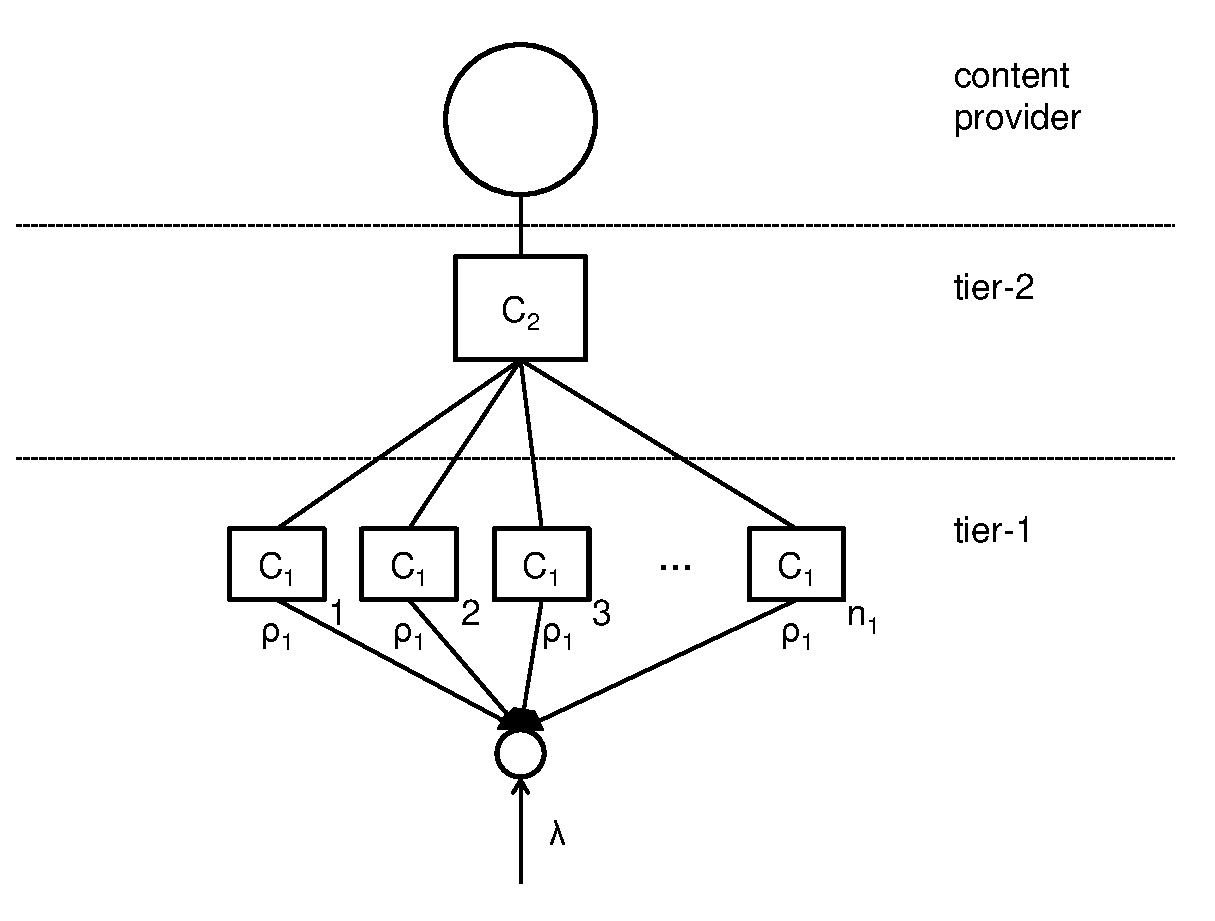
\includegraphics{cloud/figures/hcmodel}
  \caption{Stakeholders investigated in the cloud scenarios.}
  \label{fig:hcmodel}
\end{figure}

We first provide an overview of the involved stakeholders and \glspl{KPI} in \reffig{fig:cloud:model}.
If we study the operation of a machine cloud, both the cloud operator and the cloud user need to be considered.
The cloud operator is interested in increasing revenue, i.e. attracting a high number of customers, and decrease financial expenditure, e.g. by reducing consumed energy.
The customer of a cloud operator is interested in good \glspl{SLA}, for example a low delay before processing of a job can begin.
In the second scenario, the network function operator taking the role of a customer in the previous scenario, is interested in provisioning a minimal number of resources from the cloud operator, in order to reduce cost, while in turn providing a sufficient \gls{SLA} to its customers.
The users of the virtualised network functions demand a sufficient availability of the provided service.
Finally, in case of the human-cloud scenario, the cloud operator has to satisfy two stakeholders with conflicting interests.
On the one hand, employers are interested in a fast completion of the offered tasks.
On the other hand, workers are interested in obtaining a high income.
These goals are clearly conflicting, as fast completion can be obtained by providing a high number of available workers.
However, income per workers increases if the tasks are distributed between fewer workers.
Thus, the human-cloud operator has to balance the interests of the two stakeholders.

The contribution of this chapter is threefold
\begin{enumerate}
\item We provide a model for energy-efficient data centre operation and discuss sensible parameter configurations for the different stakeholders.
\item We study algorithms for resource provisioning on the example of a virtualised network function and evaluate their performance with respect to the demands of the stakeholders.
\item We model a crowdsourcing platform and provide guidelines for platform operators regarding resource acquisition.
\end{enumerate}

The content of this chapter is published in~\cite{Schwartz2012a,Metzger2014a,Schwartz2015}.
In \refsec{sec:cloud:related_work} we provide an overview of related work relevant to this chapter.
Then, in \refsec{sec:cloud:data_centers} we discuss the tradeoffs faced by a cloud operator.
We focus on the customer of a cloud operator in \refsec{sec:cloud:virtualized_network_functions} and discuss challenges when provisioning virtualised network functions.
Strategies for resource provisioning of a human-cloud are considered in \refsec{sec:cloud:crowdsourcing}.
Finally, we provide lessons learned from our studies in \refsec{sec:cloud:lessons_learned}.

\section{Background and System Description}\label{sec:aggregation:background}
In this section we describe different bandwidth aggregation approaches in praxis and present related work on the performance evaluation of bandwidth aggregation systems.
In addition, we describe our system model of bandwidth aggregation systems with offloading policy.

\subsection{Bandwidth Aggregation Approaches}\label{sec:aggregation:background:aggr}

The principle of sharing or offloading between multiple Internet access links is already widely used by commercial services as well as research work. WiFi-sharing communities like Fon\footnote{\url{http://www.fon.com}}, Karma\footnote{\url{https://yourkarma.com/}}, WeFi\footnote{\url{http://wefi.com/}}, and Boingo\footnote{\url{http://www.boingo.com/}} offer access to an alternative Internet link (WiFi instead of mobile), which provides a faster access bandwidth and reduces the load on stressed mobile networks. With respect to this so called ``WiFi offloading'', the research community investigated incentives and algorithms for access sharing \cite{mamatas2010incentives}, and ubiquitous WiFi access architectures for deployment in metropolitan areas \cite{sastry2007architecting, vidales2009metropolitan}. Moreover, \cite{lafuente2011flexible,donelson2012patent,seufert2013horst} describe systems for trust-based WiFi password sharing via an online social network (OSN) app. WiFi sharing is not a legal vacuum and a first exemplary overview on Swiss and French rights and obligations was given in \cite{camponovo2005wlan} but must be treated with caution due to international differences and interim law revisions.
The opposite concept to Wifi offloading, i.e., WiFi onloading, is presented in \cite{rossi20133gol}. The idea is to utilize different peaks in mobile and fixed networks to onload data to the mobile network to support applications on short time scales (e.g., prebuffering of videos, asymmetric data uploads).

%Bewifi
An access link sharing concept, which goes beyond pure offloading, is BeWifi, which was developed by Telefonica \cite{goma2013patent} and builds on previous works about backhaul capacity aggregation \cite{kandula2008fatvap,giustiniano2010fair}. BeWifi uses modified access points, which act as normal access points until their clients saturate more than 80\% of the backhaul capacity. Then, the access point will scan for close access points, which will provide additional bandwidth if their utilization is below 70\%. Backhaul capacity and utilization are announced by each access point via beacon frames. Instead of introducing a secondary WiFi radio, BeWifi uses time-division multiple access (TDMA) and the 802.11 network allocation vector (NAV) to connect to neighboring access points for bandwidth aggregation in a round robin fashion with a weighted proportional fairness schedule.

% The client-based solution requires driver modifications on the wireless clients.
% Each wireless client needs to feature a virtualized wireless card.
% This implies that for a commercial deployment the operating system and wireless driver of every WiFi client needs to be modified, which would produce a high amount of costs.
% %As one may realize, the cost of such an approach is absolutely prohibitive.
% The problem of the diversity of devices that need to be modified can be solved
% by deploying the aggregation scheme in the access points, which are usually provided by ISPs.
% However, current methods to perform aggregation with single-radio devices are not meant to be used in APs.
% Introducing a secondary WiFi radio in the APs could provide a technical solution, but it increases the cost of a device that is subsidized by the ISP, making the solution impracticable.

\reffig{fig:aggregation:background:aggr} shows a client-based and an access point solution for the bandwidth aggregation proposed in \cite{goma2013patent}.
The state of the art client-based system proposes to use a TDMA based access strategy for accessing selected access points in range in a round robin fashion, i.e., no concurrent data transmission via different frequencies is taking place.
The system utilizes inband signaling, a switching frequency of 100ms and requires less than 1.5ms for switching.
%The state of the art client-based aggregation schemes propose the use of TDMA to enable a single-radio client to connect to all the neighboring access points, as in \reffig{fig:aggregation:background:aggrclient} regardless of their frequency of operation. Over cycles of 100 ms the wireless client sequentially connects to all selected access points within range in a round robin fashion.
%The system utilizes inband signaling and requires less than 1.5 ms for switching.
Using the standard 802.11 power saving feature, a client is able to notify its absence to the access points it is connected to, so that they buffer packets directed to it.
A client performing aggregation appears to be sleeping in all access points but the one that is currently scheduled in the round robin cycle.
%No concurrent data transmission via different frequencies is taking place.
The access-point-based solution can be mapped to the client-based solution, if an access point acts as access point to its clients, and as a client to neighboring access points.
%single-radio AP that acts as an AP to its clients, and as a client to neighboring APs, and show that the problem can be mapped to the client-based solutions allowing the same optimization objectives

%acts as an AP and as a client of a neighboring AP
%the APs transmit on different channels
%The client-based solution is able to fully aggregate the available capacity of the
%backhaul links for a wider range of wireless channel capacities.
%their need for client modifications makes their deployment cost prohibitive.
%To unleash the potential of those solutions, the present invention provides and implements a system that can approach the benefits of client-based solutions requiring modifications only on the APs

\begin{figure*}[tb]
    \centering
    \begin{subfigure}[t]{0.5\textwidth}
        \centering
        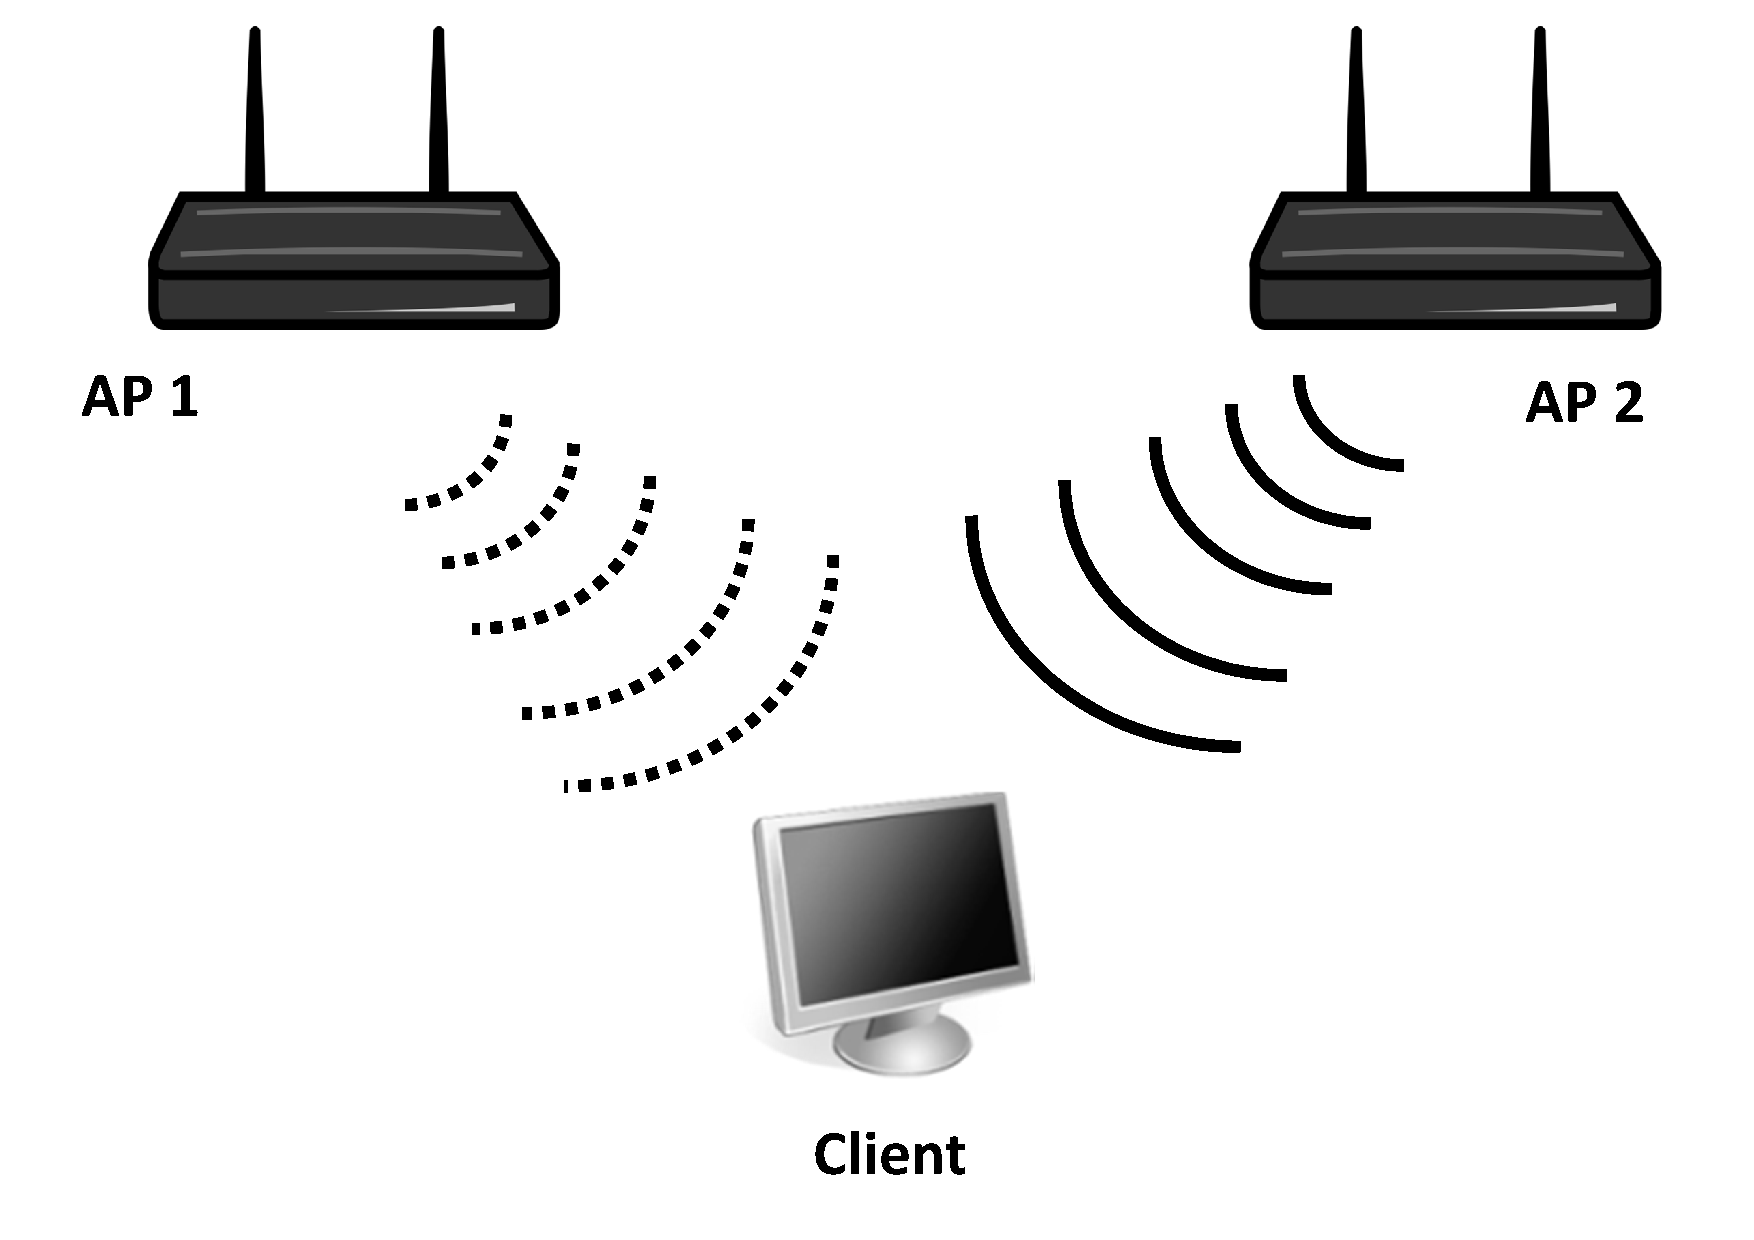
\includegraphics[width=.9\textwidth]{aggregation/background/figures/aggr_client_sw}
        \caption{Client-based}
				\label{fig:aggregation:background:aggrclient}
    \end{subfigure}%
    ~
    \begin{subfigure}[t]{0.5\textwidth}
        \centering
        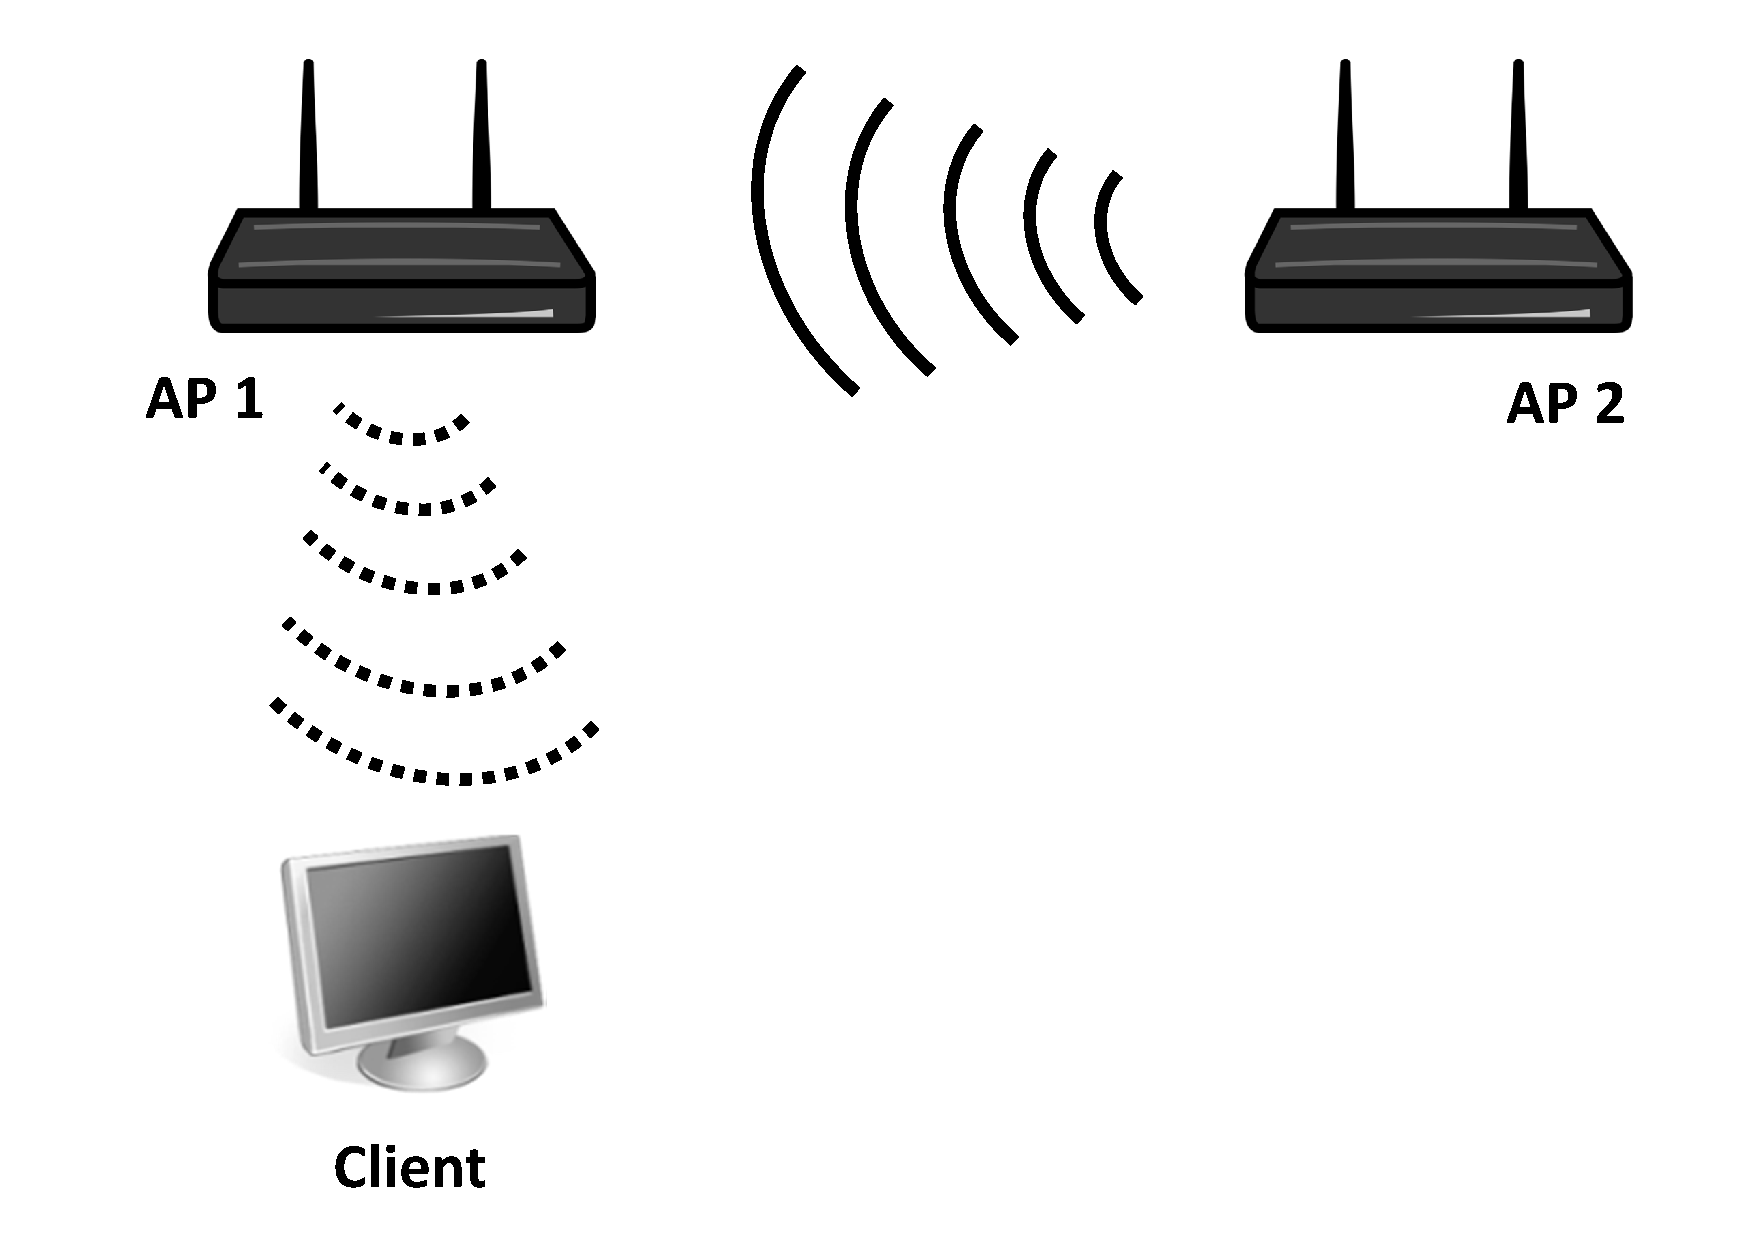
\includegraphics[width=.9\textwidth]{aggregation/background/figures/aggr_ap_sw}
        \caption{Access-point-based}
				\label{fig:aggregation:background:aggrap}
    \end{subfigure}
    \caption{Client-based and access-point-based solution for bandwidth aggregation.}
		\label{fig:aggregation:background:aggr}
\end{figure*}

From a technical perspective, bandwidth sharing and offloading are enabled by implementing handovers and/or multipath connections, which are well covered in research. \cite{gonzalez2013radio,paasch2012exploring,chen2013energy} show the feasibility of multipath TCP for handovers between mobile and WiFi networks in the current Internet and \cite{khadraoui2014survey} describes available features for mobile traffic offloading. Futhermore, \cite{gladisch2014survey} gives an overview on approaches that enable mobility and multihoming.
%In \cite{shifrin2010c3} a collaborative token bucket algorithm, which implements an effective distribution of the transmission rates is analyzed to evaluate the performance of wireless ad-hoc and mesh networks.

\subsection{Perfomance Models for Bandwidth Aggregation Systems}\label{sec:aggregation:background:models}

Theoretically, bandwidth sharing between WiFi access points can be considered as load sharing among systems.
Generally load sharing systems can be classified in partitioning, partial sharing and complete sharing systems.
Partitioning systems work completely independent from each other.
Each system has its own queue and buffer space and processes only requests arriving at its queue.
Complete sharing systems have a shared queue and buffer space. When processed, a request in the shared queue is assigned to the system which is currently least loaded.

Partial sharing systems have their own queues, but may offload requests to other systems if they are overloaded, or process requests from other overloaded systems.
Different partial sharing or complete sharing models have been investigated in literature.
In \cite{trangia1993trunk} the bandwidth usage by different services in a broadband system in complete sharing and partial sharing mode with trunk reservation is investigated.
Multidimensional Markov chains are used in \cite{chen2002performance,zhang2006dynamic,ke2010performance} to evaluate the performance of cellular network systems with different service categories.
The blocking probability of a complete sharing system has been approximated in \cite{kaufman1992blocking}.
This approximation is used in \cite{fodor2007bounding} to evaluate the performance of mobile networks with code division multiplexing supporting elastic services.
However, none of the models can be used to seamlessly evaluate the performance of systems between partitioning and complete sharing.

Thus, we develop a model based on a two dimensional Markov chain with thresholds to study the transition of blocking probabilities of partitioned, partial sharing, and complete sharing systems.
%The Markov model is limited to two access links only.
This limits its applicability, since the number of average WiFi access points visible to clients is much higher in densely-populated areas.
In densely-populated areas bandwidth of a high number of WiFi access points is aggregated. In this case an assessment with the Markov model  is not possible, since it is limited to two access links. An extension of the Markov model to $m$ dimensions would require solving an equation system with $n^m$ equations, which is computationally too complex.
Therefore, we extend the model to be applicable to multiple access links by utilizing a fixed point approximation.

The fixed point approximation is used to reduce the m-dimensional Markov chain to one dimension similar to \cite{trangia1992polling, staehle2002approximation}, where the approach is used for analytic models for polling systems and the interference distribution in UMTS networks, respectively.
The underlying Markov chain highly differs from existing fix-point approaches, since it considers support and offloading thresholds.
To the best of our knowledge this is also the first work that considers an inner and an outer composite system to apply the fixed point analysis in heterogeneous load conditions.

%multipath transmissions
%Multipath transmissions?
%von hossi:
% Survey on Mobility and Multihoming in Future Internet: http://link.springer.com/article/10.1007/s11277-012-0898-6#page-1
% A Survey of Available Features for Mobile Traffic Offload: http://ieeexplore.ieee.org/stamp/stamp.jsp?tp=&arnumber=6843152
% Exploring Mobile/WiFi Handover with Multipath TCP: http://inl.info.ucl.ac.be/system/files/cell06-paasch.pdf
% An Energy-aware Multipath-TCP-based Content Delivery Scheme in Heterogeneous Wireless Networks: http://www.eeng.dcu.ie/~munteang/papers/2013_WCNC_SC.pdf
% Radio access considerations for data offloading with multipath TCP in cellular/WiFi networks: http://ieeexplore.ieee.org/xpl/freeabs_all.jsp?arnumber=6496709&abstractAccess=no&userType=inst

\subsection{System Model}


For simplicity and mathematical tractability we make assumptions on the link capacities and the service rates of bandwidth fractions. This allows analytic performance evaluation of bandwidth aggregation systems with offloading policy and understanding its characteristics.


%\newtheorem{amp4}[amp1]{Assumption}\label{amp:traffic}
%\begin{amp4}
%	The arrivals of traffic bursts follow a Poisson process.
%\end{amp4}

%There are different effects in real systems, which are not considered in the model.

\newtheorem{amp1}{Assumption}\label{amp:switching}
\begin{amp1}
	The switching time to another access link is zero.
\end{amp1}
In practice, TDMA is used to aggregate the bandwidth of two access points operating on different channels.
During the time in which the client is switching frequencies, it cannot send or transmit data. This time is called switching time and for state of the art systems it is 1.5ms \cite{goma2013patent}.
This switching time slightly decreases the effective throughput of the system.
Signaling among the cooperating access points is necessary to report the current load and the offloading state.
The messages exchanged produce a signaling overhead, which can limit the performance of the system.
In practice APs announce their backhaul link capacity through Beacon frames, as well as their available-for-aggregation throughput, i.e. the part of their capacity that is not utilized by their clients \cite{goma2013patent}.
However, in \cite{goma2013patent} the aggregate throughput remains almost constant across the different experiments, indicating that the overhead of switching and signaling is fixed and only slightly impacts the overall throughput.
\newtheorem{amp2}[amp1]{Assumption}\label{amp:aggrlimit}
\begin{amp2}
	The wireless channels are clean.
\end{amp2}
Interference can limit the capacity of the wireless links.
The effect of the channel quality on the aggregation capacity is evaluated in \cite{goma2013patent}.
To account for a bad channel quality in our model, the link capacity can be reduced accordingly.

\newtheorem{amp3}[amp1]{Assumption}\label{amp:servicetimes}
\begin{amp3}
	The service time of bandwidth fractions follows a negative exponential distribution.
\end{amp3}
%In practice, the link throughput has low variations which makes the service time of traffic bursts more deterministic.
%As shown in \cite{burger2016phycom} for two cooperating systems, the Markov model also provides good approximations for the received bandwidth and blocking probability for deterministic and highly variant service time distributions.

%%We think that these effects are marginal and negligible on high loads.
%As these effects have only marginal impact on the system performance, they are neglected in the model.
%By making the assumptions, we can evaluate the performance of bandwidth aggregation systems with offloading policies analytically and understand its characteristics.

%develop a solution that can enable the desired functionality simply through software AP modifications and without any client support

%a single-radio AP that acts as an AP to its clients, and as a client to neighboring APs, and show that the problem can be mapped to the client-based solutions allowing the same optimization objectives,

%More importantly, if the two metrics are add up, the aggregate throughput remains almost constant across the different experiments, indicating that the overhead of switching from AP to client is fixed and only impacts overall aggregate throughput by 3.2 Mbps

%This value is actually w11switching=0:86 xW11-No-Switching. This shows the impact of the channel switching overhead.

%potential of those solutions, the present invention provides and implements a system that can approach the benefits of client-based solutions requiring modifications only on the APs.

%\subsection{Model Limitations}
%
%The model has limitations. A critical part of the model are the negative exponential service times, which may in reality be more deterministic, since the link throughput has low variations.
%However, as will be shown in section \ref{sec:simgeneral} the model also provides good approximations for the received bandwidth and blocking probability for different service time distributions.
%There are different effects in real systems, which are not considered in the model.
%For example signaling among the cooperating access points is necessary to report the current load and the offloading state.
%The messages exchanged produce a signaling overhead which can limit the performance of the system.

%To use Markov chain model analysis, we assume in the following that the processes
We model the load on $m\geq 2$ access links as depicted in Figure~\ref{fig:aggr:sysmodel}. The throughput of each Internet connection is limited by a bottleneck (either on application side, on server side, or in the core Internet), such that single connections will utilize a certain share of the access link bandwidth. Therefore, the available capacity of a link $c$ is divided into a number $n$ of small atomic bandwidth fractions of equal size. This means, $c = n\cdot \xi$ with a global constant $\xi$ denoting the granularity of bandwidth allocation. Thus, different capacities $c_i$ are modeled by assigning different $n_i$ to the links.

\begin{figure}[tb]
	\centering
 	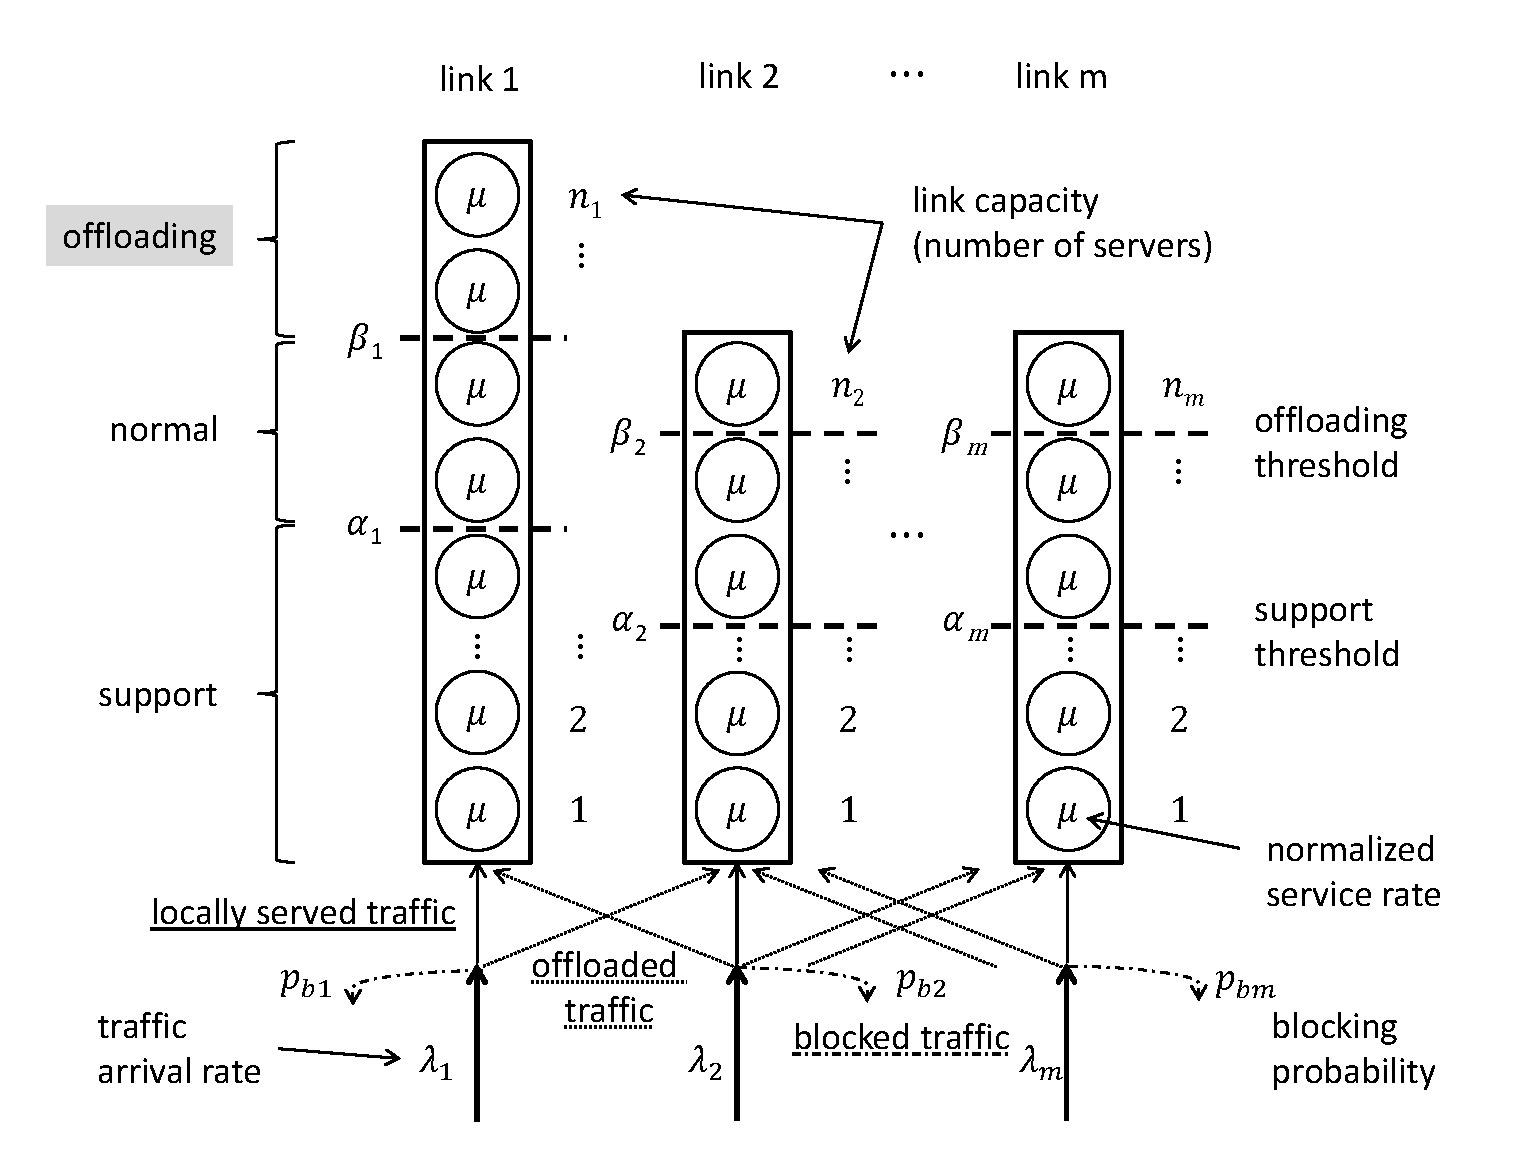
\includegraphics[width=0.9\textwidth]{aggregation/performance_model/figures/model_m}
  	\caption{System model.}
  	\label{fig:aggr:sysmodel}
\end{figure}

%In our scenario, we look at loaded access links on a short time scale. The throughput of each Internet connection is limited by a bottleneck (either on application side, on server side, or in the core Internet), such that the capacity of an access link cannot be fully utilized by a single connection. This means, each Internet connection will utilize a certain share of the access link bandwidth. The available capacity of a link $c$ is divided into a number $n$ of small atomic bandwidth fractions of equal size. This means, $c = n\cdot \xi$ with $\xi$ resembling the granularity of bandwidth allocation. For example, a $c=10\ \text{Mbps}$ link can be modeled as $n=20$ bandwidth fractions of $\xi=500\ \text{kbps}$ each, or also as $n=100$ bandwidth fractions of $\xi=100\ \text{kbps}$ each. For the remainder of this paper, we will consider $\xi$ as a global constant in the given scenario and model different capacities $c_i$ by assigning different $n_i$ to the links.
%short time frame load on links can be as stationary small variations poisson process

We consider the system in a short time frame, where the system load can be considered stationary.
Each access link is modeled as a multi-server blocking system, in which each server represents an available bandwidth fraction of the link.
Its utilization variations are modeled as a stationary process of singular and independent arrivals of traffic bursts, i.e., bandwidth fraction requests. This allows modeling an access link as M/M/n loss system \cite{kleinrock1975queuing}. We define $X$ as the random variable of the number of occupied bandwidth fractions on each backhaul link. It is modeled by a birth-death-process, in which bandwidth fractions are requested with Poisson arrivals at rate $\lambda$ and occupied for an negative-exponentially distributed service time with globally normalized rate $\mu=1$. Consequently, the load on each link is given by $\rho=\frac{\lambda}{n\cdot \mu}=\frac{\lambda}{n}$. The probability that $k$ bandwidth fractions are occupied in the considered M/M/n queue is $x(k)=P(X=k)$.

In the BeWifi approach (cf.~\refsec{sec:aggregation:background:aggr}), two thresholds are used, which define the bandwidth aggregation/offloading policy. The support threshold $\alpha$ indicates up to which percentage of utilization (i.e., number of own occupied bandwidth fractions) the system will offer bandwidth fractions to other systems. Furthermore, the offloading threshold $\beta$ with $\alpha\leq\beta$ sets the percentage of utilization above which the system will try to use bandwidth of other systems. According to these thresholds, a system can be in one of the following three macro states:

\begin{enumerate}
	\item \textit{support} ($0 \leq X < \lfloor\alpha\cdot n\rfloor$):\\ low utilization and offering bandwidth \, ,
	\item \textit{normal} ($\lfloor\alpha\cdot n\rfloor \leq X < \lfloor\beta\cdot n\rfloor$):\\ normal operation \, ,
	\item \textit{offloading} ($\lfloor\beta\cdot n\rfloor \leq X \leq n$):\\ high utilization and offloading to other systems \, .
\end{enumerate}

By applying the offloading policies, different Internet access links will collaborate and share traffic. More details on the investigated scenarios are presented in the following section.

Two bandwidth aggregation systems, i.e., systems offloading between $m$ access links, will be analyzed. First, we consider a bandwidth aggregation system with equal load on each access link. Moreover, a system in which one access link has a different load than the other $m-1$ links is modeled. As reference system we considered partitioned systems without offloading.% and a complete sharing system.

\subsection{Analysis of Reference Systems}

We compare the bandwidth aggregation gain of multiple collaborating Internet access links to a partitioned system without offloading. %, although it has to be noted that in many practical cases complete sharing is physically not possible.
The received bandwidth of each access link $E[X_i]$ and the blocking probability $p_{b_i}$ of each system $i$ are evaluated. The blocking probability gives the probability that the link is fully utilized and a bandwidth request of an application cannot be entirely satisfied. In practice, if TCP is used on the access link, the Internet connections throttle themselves and share the link equally. Depending on the used application and its characteristics, the application performance can then suffer, which can result in user dissatisfaction.

\subsubsection{Partitioned and Complete Sharing Systems}

For completely partitioned systems, i.e., $m$ different M/M/$n_i$ loss systems with arrival rates $\lambda_i,\ i\in\{1,\ldots, m\}$, the received bandwidths $E_0[X_i]$ can be computed individually for each access link by Little's Theorem as
\begin{equation}
E_0[X_i] = \frac{\lambda_i}{\mu}\cdot(1-p_{b_i}),% = \lambda_i\cdot(1-p_{b_i})\ ,
\end{equation}
in which we use the rate of accepted arrivals $\lambda_i\cdot(1-p_{b_i})$ and the globally normalized service rate $\mu=1$.

The blocking probability of partitioned systems $p_{b_i}$ follows from the Erlang-B formula \cite{kleinrock1975queuing}
\begin{equation}
p_{b_i} = \frac{\frac{(\frac{\lambda_i}{\mu})^{n_i}}{n_i!}}{\sum_{k=0}^{n_i}\frac{(\frac{\lambda_i}{\mu})^{k}}{k!}}\ .
\end{equation}

The performance $E_s[X]$ of a complete sharing system, i.e., a single M/M/n loss system with $n=\sum_{i=1}^m n_i$ servers and an arrival rate of $\lambda=\sum{i=1}^m \lambda_i$, can be computed by the same formulae.

\subsubsection{Approximations and Performance Metrics}

An approximation $\tilde{p}_b$ of the blocking probability $p_b$ can be calculated by the joint probability of a single system being fully occupied, while a separate single system is above the support threshold $\alpha$, i.e. could not help. If $X_1$ and $X_2$ are random variables for the number of jobs in system 1 and system 2, the joint probability is

\begin{equation}
\tilde{p}_b = P(X_1=n_1,X_2\geq \alpha\cdot n_2) = P(X_1=n_1)\cdot P(X_2\geq \alpha\cdot n_2)\ .
\end{equation}

Moreover, we analyze the mean total number of occupied bandwidth fractions $E[X]$% as well as the mean number of occupied bandwidth fractions $E[X_i]$ of each system
, which corresponds to the mean of total aggregated bandwidth. Following the same argumentation as above, $E[X]$ can be computed by Little's Theorem as
\begin{equation}
E[X] = \frac{\lambda_1+\lambda_2}{\mu}\cdot (1-p_b) = \frac{\lambda_1}{\mu}\cdot (1-p_{b_1})+\frac{\lambda_2}{\mu}\cdot(1-p_{b_2})\ .
\end{equation}

Finally, we take a look at the received bandwidth at each access link $E[X_{A_i}]$. Thereby, $X_{A_i}$ is a random variable for the number of bandwidth fractions (in all systems), which are occupied by arrivals from system $i$. It is obvious that $E[X_{A_i}] = E[X_i]
 = E_0[X_i]$ for the partitioned system. In case of offloading, $E[X_{A_i}]$ can be calculated from the mean total number of occupied bandwidth fractions by taking into account the share of accepted requests from each system.
\begin{equation}\label{equ:gain}
E[X_{A_i}] = \frac{\lambda_i(1-p_{b_i})}{\lambda_1(1-p_{b_1})+\lambda_2(1-p_{b_2})}\cdot E[X] = \frac{\lambda_i}{\mu}\cdot (1-p_{b_i})
\end{equation}

Nevertheless, it is the goal of bandwidth aggregation to cooperate in order to use spare capacity on access links to increase the received bandwidth where needed. Therefore, we can quantify the percentage of bandwidth gain for each system as
\begin{equation}
\omega_i = \frac{E[X_{A_i}]-E_0[X_i]}{E_0[X_i]}\ .
\end{equation}

\subsection{Simulation Description}
A discrete-event based simulation using arrival and departure events is implemented to validate the analytic model and to assess the system performance in more general cases. Each of the $m$ systems has a Poisson arrival process with rate according to its load. The service time of bandwidth fractions is exponentially distributed with mean 1. Offloading decisions are made according to the the number of occupied bandwidth fractions in the systems with respect to the support and offloading threshold. Therefore, the simulation state holds the requests being processed and the number of occupied bandwidth fractions for each system.

\section{Simulative Evaluation of Hierarchical Caching Systems}\label{sec:hierarchical:simulative:simulative}

We develop an event-based simulation framework to evaluate the performance of content delivery networks.
The results derived from the simulative evaluation are used to validate the analytic models.
The simulation framework further allows to consider complex system characteristics in the performance evaluation that are not covered by the analytic models, such as the transit costs charged on inter-domain links.

A hierarchical content delivery network with bandwidth constraints has been evaluated by simulation in \cite{applegate2010optimal}.
The impact of using edge resources with limited capacity for content delivery on QoE is evaluated by means of simulation in \cite{info3-inproceedings-2015-530}.
In the following we describe the simulation model and investigate the benefit of overlays networks in hierarchical caching systems.
We use the model for transit traffic, c.f. \refsec{sec:p2p:methodology}, to assess the potential to save costs produced by inter-domain traffic.

\subsection{Simulation Model}\label{sec:simeval}

The parameters considered in the content delivery simulation framework are
\begin{enumerate}
  \itemsep0em
  \item the resource distribution,
  \item the caching and content placement strategy,
  \item the resource selection strategy,
  \item the content demand,
  \item the AS-Topology.
\end{enumerate}
Other considered parameters that are not relevant for this monograph, are
\begin{enumerate}
  \itemsep0em
  \item the social network of users,
  \item the video bitrate and chunk-size distribution,
  \item and the application and QoE.
\end{enumerate}
In the following we briefly describe each of the parameter sets and provide models.

\subsubsection{Resource Distribution}
The resource distribution determines how video streaming sources are distributed among autonomous systems.
The number and size of autonomous systems is specified.
The size of an autonomous system is given by the number of end-users located in it.
In literature, the distribution of end-users on ASs is characterized as heterogeneous \cite{Hossfeld2011}.
We use a geometric distribution as a basic model for number of end-users in the ASs.
A more detailed model is developed using the Internet Census dataset, c.f. \refsec{sec:aslevel:census}.
Video streaming sources can be a) data centers of the content provider, b) edge caches of the content provider, c) caches hosted by the ISP, d) home router / NaDas, or e) end-user devices.
For each video streaming source the AS-location and its capacity is specified.
The capacity is given by the number of items that can be cached.
The size of the item catalogue is also specified in this parameter set.

The cache resource can have bandwidth constraints specified by the mean and the standard deviation of the upload bandwidth.
If the upload bandwidth of a cache is limited, the service time of an object is calculated according to the available bandwidth and the object size.
The service times of the objects served by a cache are updated if the upload bandwidth changes or if an object request arrives or is completed.
A cache can block requests if the available bandwidth is below a certain threshold, or if the cache is busy serving a request.

\subsubsection{Caching and Content Placement Strategy}
The caching and content placement strategy determines in which video streaming source which video item is placed and when.
The content placement strategy is defined by the caching strategies of the individual caches.
In a distributed approach each cache decides based on the information it has which items to cache.
If global knowledge of the item demand is assumed, optimized content placement strategies such as hot warm cold.
Thus, the availability of items in ASs might for example be increased.
Each caching strategy is further defined by its specific parameters according to \refsec{sec:hierarchical:background:strategies}.

\subsubsection{Resource Selection Strategy}
The resource selection strategy determines from which cache instance an item is streamed when requested.
The simplest resource selection just selects a random resource.
By default, resources in tier-1 are selected first in hierarchical content delivery networks.
Other resource selection strategies that try to optimize different metrics were implemented, such as local resource selection, which tries to save inter-domain traffic by prioritizing caches in the order: home router / NaDa in the same AS, ISP managed cache in the same AS, edge cache of content provider, data center of content provider.
%Further resource selection strategies that are not yet implemented could for example consider load balancing of the request based on the capacity of the caches.

\subsubsection{Social Network of Users}
The social network of users determines the friendship relationships between users. A basic model only defines the number of users in the system.
The number of friends of the user can be modeled by a power-law or geometric distribution.
A more detailed model specifies the friendship graph which consists of a node for each user and edges between users with friend relationships.
Friendship graphs have typical properties, such as a heavy-tailed in and out degree distribution.
In literature are different models for generating graphs with these properties.
A model used to generate social network graphs with varying size and density is the forest fire model \cite{leskovec2005graphs}.
We further specify the feed size as parameter that represents the news feed of social network platforms.
The news feed is updated in sharing events.
Videos which are on the news feed of a user are watched with high probability.
Categories are defined by specifying the probability that a user is interested in a particular category.

\subsubsection{Traffic and Popularity Model}
The content demand determines the request rates of the video items.
Different demand models are implemented in the simulation, that reach from basic models that only consider the popularity distribution of the items to detailed models that consider temporal, spatial and social dynamics, c.f. \refsec{sec:hierarchical:background:traffic}.

The arrival process of video requests is specified by the inter-arrival time of video requests.
The request rate depends on the time of day and is generally lower at night.
The day is divided in short time slots, where the arrival rate does not change significantly, so that the arrival process can be assumed as quasi stationary.
In these time slots the arrival process is modeled as Poisson-process.
The parameter lambda of the arrival process depends on the popularity of the item and the time of day.
The probability of sharing a watched video is given by the sharing probability.

\subsubsection{Autonomous System Topology}
In order to estimate the amount of inter-domain traffic and transit costs produced, and AS topology with AS paths can be specified.
The AS paths connect the caches and data centers providing the content with the users consuming the content.
For that purpose the AS paths are inferred from AS relationships as in \refsec{sec:p2p:methodology}.
Assuming that the number of users is proportional to the number of IP addresses in an AS, we use the results of the Internet Census Dataset evaluation in \refsec{sec:aslevel:census}, to determine the distribution of users on ASs, which has to be specified.

Finally, Simulation parameters are specified that define the random number seed, the simulation time and the parameter study.

\subsubsection{Performance metrics}

To assess the performance of content delivery networks several metrics are considered:

\begin{enumerate}
\item Cache hit rate: The ratio of requests to a cache that find the object in the cache (cache hit).
\item Cache serve rate: The ratio of requests to a cache that find the object in the cache and that are not blocked due to bandwidth constraints.
\item Cache contribution: The share of all requests that is served by a cache.
\item Inter-domain traffic: The share of requests by users in an AS that can not be served by a cache in the same AS.
\end{enumerate}

\begin{figure}[bt]
  \centering
  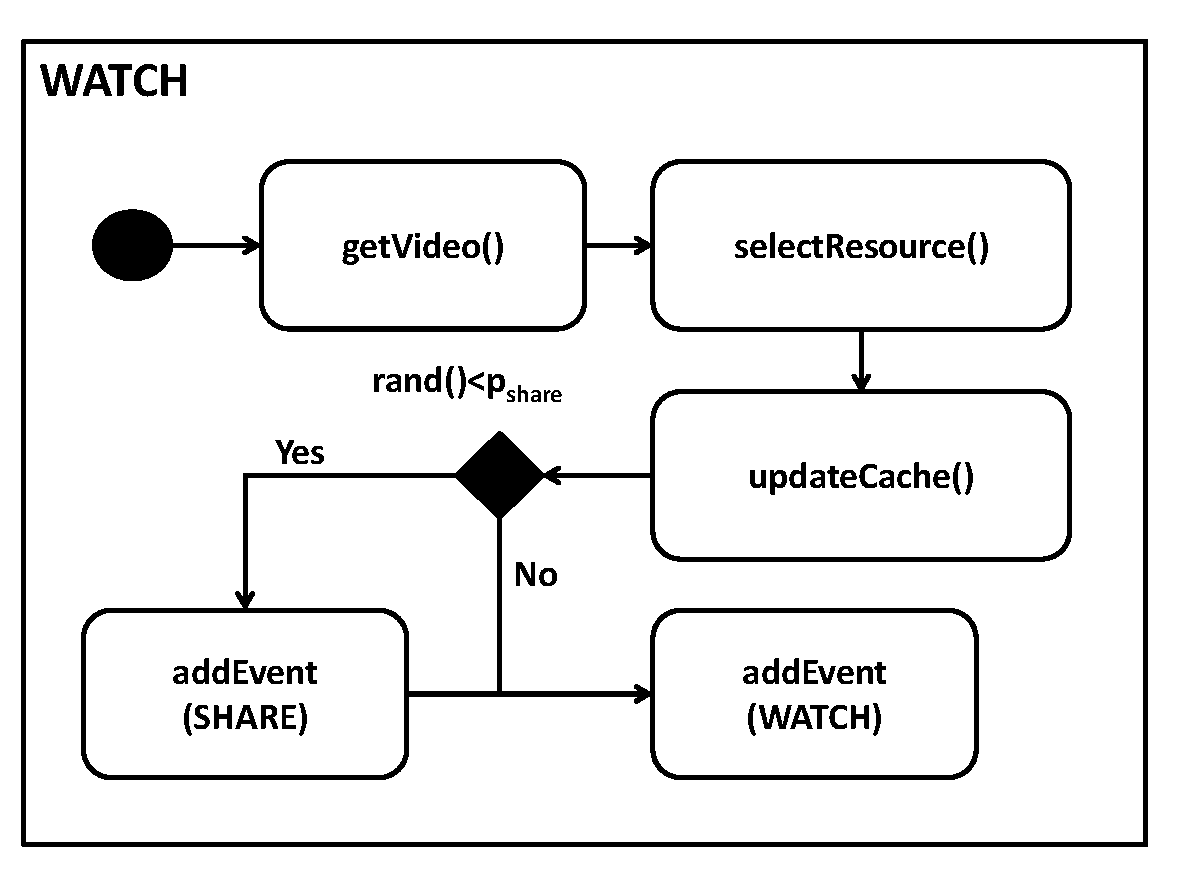
\includegraphics[width=0.6\textwidth]{hierarchical/simulative/figures/watch}
  \caption{Proccess diagram of a WATCH event.}
  \label{fig:WATCH}
\end{figure}

The content delivery simulation framework is implemented in MatLab.
The simulation is event-based including two major events.
First there is the WATCH event, which is processed when a user watches or consumes a video item.
Second there is a SHARE event, which simulates a sharing action of a user, where the video is posted on the news feeds in the social network.
\reffig{fig:WATCH} shows the process diagram of a WATCH event.
The process of a WATCH event starts by selecting a video dependent on the demand model specified in the parameters.
A video with video identifier $v_\text{id}$ is returned.
In the next step a cache or data center is selected that holds the item with $v_\text{id}$.
The download of the item from this resource is recorded in the statistics.
The cache identifier $c_\text{id}$ is returned and the cached items are updated according to the caching strategy specified in the parameters.
The user then decides to share $v_\text{id}$ with probability $p_\text{share}$.
In this case a SHARE event is added.
Finally, the next WATCH event is added according to the traffic and popularity model.

A SHARE event puts a given $v_\text{id}$, or a random video according to the user's interest on top of the news feed of the user's friends.
The user's friends are determined by the social graph.
The simulation is initialized with a WATCH event for each user.

The simulation framework is open source and available on github\footnote{\url{https://github.com/pettitor/content_delivery}}.

\input{hierarchical/analytic/analytic}
\section{Analysis of Caching Systems with Bandwidth Constraints}\label{sec:model}

In order to evaluate content delivery networks based on the number of available home gateways and their limited capacity, we define a system model for a tiered caching architecture.
Tier-1 caches are on leaf nodes such as NaDas, caches of the content delivery network are in tier-2 and ultimately tier-3 is the content provider.
We use analytic models to calculate the efficiency of the tiered caching architecture.


%\subsection{Performance Metrics}

%\begin{itemize}
%	\item hit rate, define as hit on device WITH enough available bandwidth / resources
%	\item effective cache capacity
%  \item ...
%\end{itemize}

%To be able to estimate the costs for ASes arising from transit services, we need to know how much traffic is generated and how much providers charge customers for forwarding the traffic.
%We consider a snapshot and assume instantaneous traffic rates, i.e., the file-size of the download can be neglected.
%For simplicity we make assumptions on how much traffic is generated in each swarm, depending on the the number and location of peers.
%\newtheorem{A}{Assumption}\begin{A}\label{npeers}
%The traffic generated by a peer is equally shared among its neighbors.
%\end{A}
%\newtheorem{B}[A]{Assumption}\begin{B}\label{ntraffic}
%All peers generate traffic at the same rate.
%\end{B}
%\newtheorem{C}[A]{Assumption}\begin{C}\label{npaths}
%The traffic between ASes is equally shared among the paths that connect them.
%\end{C}
%In practice traffic rates are allocated by BitTorrent's choking algorithm and traffic is generally not shared among different AS paths. But, since we consider the aggregated traffic of a large number of swarms, we argue that these assumptions are reasonable and that the results are not changed significantly.

\subsection{Analytic Performance Models for Caching Systems}

In the following we provide analytic models to evaluate the performance of a tiered caching architecture.
We use existing models for systems without bandwidth constraints in order to determine baselines and upper bounds for comparison.
We then show our approach to determine the hit rate of hierarchical cache networks with bandwidth constraints.

\subsubsection{The Che Approximation}

\subsubsection{No bandwidth constraints}

The baseline is given by the cache hit rate of the tier-2 cache without tier-1 cache support $p'_\text{hit}(2)$ using the Che approximation for the LRU cache hit rate. The characteristic time $T_{C_2}$ depends on the capacity of the tier-2 cache $C_2$ and is determined by a fixed point approximation according to \cite{che2002hierarchical}.
Due to the memoryless property of the Markov process the hit probability equals the stationary probability that an item $m$ is in the cache.

\begin{equation}
p_\text{hit}(2,m)=p_\text{in}(2,m)=1-e^{-\lambda_{m}T_{C_2}}
\end{equation}

The overall hit probability in tier-2 is calculated by considering the probability $p_m$ of requesting item $m$.

\begin{equation}
p'_\text{hit}(2)=\sum_m p_m p_\text{hit}(2,m)
\end{equation}
%\begin{equation}
%p_m=\frac{\lambda_m}{\sum_i \lambda_i}
%\end{equation}

To calculate the maximum hit rate for LRU, we assume that tier-1 caches are completely organized with the tier-2 cache, and the capacity of tier-1 caches is added to the tier-2 cache capacity.

\begin{equation}
\hat p_\text{hit}(m)=\hat p_\text{in}(m)=1-e^{-\lambda_{m}T_{(C_2+n_1\cdot C_{1})}}
\end{equation}

It is practically not feasible to control the capacity of all tier-1 caches and coordinate them with the tier-2 cache.
To still bundle the capacity of the tier-2 caches, the caches can form an overlay.

%The probability to find object $m$ in a tier-2 cache is $p_{in}(2,m)$.

%TODO tree case.

%\begin{equation}
%p_\text{hit}(2,m)=p_{in}(2,m)=1-e^{-\lambda_{m}T_{C_2}}
%\end{equation}

If an overlay is used, the requests that cannot be served by the personal tier-1 cache are forwarded to other tier-1 caches in the overlay, before they are forwarded to the tier-2 cache.
%The requests that are forwarded to the tier-1 cache have looked up the object $m$ in all tier-2 caches.
%The requests for object $m$ forwarded to tier-1 $\lambda_m^o(1)$ are not hit by any of the $n_2\approx p_{share}\cdot n_{user}$ tier-2 caches.

We approximate the hit rate of the overlay by calculating the hit rate of a tandem network with two caches according to \cite{martina2014unified}. The tandem network consists of the tier-2 cache and a cache that has the sum of capacities of tier-1 caches. The miss stream of the consolidated tier-1 cache is forwarded to the tier-2 cache.
The replacement strategy in the network is leave-copy-down, that means that an item is only placed in a cache if it is found in a higher tier cache. Thus only frequently requested items are propagated to lower tier-caches, which makes them more efficient. The Che approximation can be applied to tandem networks by determining $p_\text{in}(1,m)$ for the tier-1 caches.

\begin{equation}
p_\text{in}(1,m) = 1-e^{\lambda(1,m)T_{n_1 C_1}}
\end{equation}

The hit probability is no longer equal to the probability that an item is in the cache, as the cache miss stream arriving at the tier-2 cache is no longer Markov. According to \cite{martina2014unified} the hit probability can then be determined by:

\begin{multline}
p_\text{hit}(1,m) = ((1-p_\text{in}(1,m))p_\text{hit}(2,m) + p_\text{in}(1,m)) \\ \cdot(1-e^{\lambda(1,m)T_{n_1 C_1}})
\end{multline}

The rate of the miss stream $\lambda(2,m)$ arriving at the tier-2 cache can then be determined as

\begin{equation}
\lambda(2,m) = (1-p_\text{in}(1,m))\lambda(1,m) \, .
\end{equation}

The probability that an item is in the tier-2 cache is approximated assuming exponentially distributed inter request times.

\begin{equation}
p_\text{hit}(2,m) = p_\text{in}(2,m) = 1-e^{\lambda(2,m)T_{C_2}}
\end{equation}

The total hit rate in tier-$i$ is then calculated by considering the probability of an item $m$ being requested at tier-$i$ cache $p(i,m)$.

\begin{equation}
p_\text{hit}(i) = \sum_{m}p(i,m)p_\text{hit}(i,m), i\in\{1,2\}
\end{equation}
%if tC(2) > tC(1)
%   phit(2,:) = (1-exp(-l(2,:).*(tC(2)-tC(1))))+(1-phit(2,:)).*(1-exp(-l(1,:)*tC(1)));
%else
%   phit(2,:) = (1-phit(2,:)).*(1-exp(-l(1,:)*tC(2)));
%end

% wrong
%\begin{equation}
%\lambda_m^o(1)=\lambda_m\cdot(1-p_\text{hit}(2,m))^{n_2}
%\end{equation}

%The hit rate of the object $m$ in tier-1 cache in the overlay case $p_\text{hit}^{o}(1,m)$ can be approximated according to \cite{•}.

%\begin{equation}
%p_\text{hit}^{o}(1,m) \approx 1-e^{A_1^o(m)}
%\end{equation}

%where (TODO improve)
%\begin{align*}
%A_1^o(m)&=\frac 1 {n_2}\cdot \lambda_m\cdot (1-p_{in}(2,m))^{n_2}\cdot max(0,T_{C_1}-T_{C_2}) + \\ &\frac {n_2-1}{n_2}\cdot \lambda_m\cdot(1-p_{in}(2,m))^{n_2}\cdot T_{C_1}
%\end{align*}

%The hit rate of the tier-2 overlay caches $p_\text{hit}^{o}(2,m)$ is the probability of the event complementary to no tier-2 cache hit.

%\begin{equation}
%p_\text{hit}^{o}(2,m) = \lambda_m\cdot (1-(1-p_{in}(2,m))^{n_2})
%\end{equation}

The overall hit rate of the hierarchical caching system is then calculated by

\begin{equation}
\bar{p}_\text{hit} = p_\text{hit}(1)+(1-p_\text{hit}(1))p_\text{hit}(2) \, .
\end{equation}

%with $p_m=\frac{\lambda_m}{\sum_i \lambda_i}$.

\subsection{Analytic Model with Bandwidth Constraints}

The above hit rates only apply if tier-1 and tier-2 caches have unlimited bandwidth, which is practically not feasible.
Considering the home gateway scenario, the bandwidth of tier-1 caches is limited depending on the subscription and the availability of DSL.
We use the throughput of the tier-1 caches $\rho_1$ as parameter to specify the upload bandwidth available on home gateways.

%\begin{equation}
%\bar b = \frac 1 N \sum_{m=1}^N b_m
%\end{equation}

%\begin{equation}
%\bar \rho_1 = \frac 1 {n_1} \sum_{i=1}^{n_1} \rho_1(i)
%\end{equation}

%\begin{equation}
%\bar\mu = \frac{\bar b}{\bar \rho_2}
%\end{equation}

The offered traffic of item $m$ at tier-1 cache $k$ can be calculated by the quotient of the arrival rate per cache $\frac{\lambda_m}{n_1}$ and the mean service rate, which is determined by the bitrate $b_m$ and the duration $d_m$ and the link throughput $\rho_1$ in case of video contents.

\begin{equation}
a(m,k) = \frac{\lambda_m \cdot b_m \cdot d_m}{n_1\cdot \rho_1(k)}
\end{equation}

The total offered traffic of item $m$ is $a(m) = \sum_k a(m,k)$.

%\begin{equation}
%a(m) = \sum_k a(m,k) \, .
%\end{equation}

The content placement in tier-1 is specified by $X: N \times n_1\mapsto {0,1}, X(m,k) = 1$, if content $m$ is placed on cache $k$, else $0$.

According to \cite{valancius2009greening} an optimal placement of items in terms of minimum loss rate in the stationary case is achieved by the hot-warm-cold content placement.
Hot content with $a(m)\geq n_1$ is placed on each cache.
Warm content is placed on $\lfloor a(m) \rfloor$ caches.
Cold content is not placed on any of the caches.
The constraint  $\forall k, \sum_m X(m,k)\leq C_1(k)$ has to be met.
%hotwarmcold: while $\forall k, \sum_m X(m,k)\leq C_1(k)$
%\begin{itemize}
%	\item $\forall k, X(m,k)=1, \text{if}\ a(m) \geq \sum_k C_1(k) $
%	\item $\forall i, X(m,k)=1, i$ not occ TODO
%\end{itemize}

% We define the indicator function $\chi_m$ to determine if item $m$ is cached.
%
% \begin{equation}
% \chi_m =
% 	\begin{cases}
% 		1, & \exists k : X(m,k)=1 \\
%       		0, & \text{otherwise}
% 	\end{cases}
% \end{equation}

%The hit rate of the placement can be calculated by
%%TODO correct?
%\begin{equation}
%	p_\text{hit}^\text{hwc}(2,m) = \chi_m \cdot (1-\max(0,\frac{a(m)}{n_2}-1))
%\end{equation}

%and

%\begin{equation}
%	p_\text{hit}^\text{hwc}(2) = p_\text{hit}^\text{hwc}(2,m) \cdot p_m \, .
%\end{equation}

%TODO leave out
% The effective cache size of tier-1 $C_1^*$ is defined as the number of different items that is stored in tier-1 caches. It is calculated by
%
% \begin{equation}
% C_1^* = \sum_m \chi_m \, .
% \end{equation}

Since not every hit can be served by tier-1 caches because of their limited bandwidth, we consider the loss rate $p_{b}(1,m)$, which is defined as the share of requests of item $m$ that is not hit in tier-1 or is blocked if none of the tier-1 caches storing the requested item has enough bandwidth left to serve the request.

Let $\nu_m$ be the number of tier-1 caches that hold item $m$.

\begin{equation}
\nu_m=\sum_{k=1}^{n_1} X(m,k)
\end{equation}

%An item is not hit, if it is not placed in any of the tier-1, hence, if $X(m,k)=0 \forall k\in {1,\ldots,n_1}$.
An item is not hit, if it is not placed in any tier-1 cache, i.e., if $\nu_m=0$.
If an item is placed in at least one of the tier-1 caches, i.e., $\nu_m>0$, we approximate the blocking probability by the Erlang formula for a loss system with $\nu_m$ servers with mean service rate $\mu_{m} = \frac{\rho_1}{b_m\cdot d_m}$ and arrival rate $C_1\lambda_m$:


\begin{equation}
p_{b}(1,m) =
	\begin{cases}
		\frac{\frac{a_m^{\nu_m}}{m!}}{\sum_{k=0}^{\nu_m}\frac{a_m^k}{k!}}, & \nu_m>0 \\
    1, & \text{otherwise} \, ,
	\end{cases}
\end{equation}

where we approximate the offer of item $m$ with
\begin{equation}
a_m \approx \frac{\lambda_m\cdot C_1}{\mu_m} \, .
\end{equation}
Note, that here we assume that the arrival rate of requests of the $C_1$ items stored in the cache is equal to the rate of item $m$.
In order to calculate the exact stationary distribution of the blocking probability, the arrival rate of requests has to be conditioned on the feasibility of the content placement, which is too complex to evaluate.
Refer to \cite{tan2013optimal} for details.
%We also tried other arrival rates, such as average arrival rate of the items cached, which did not improve the approximation.

The blocked requests are forwarded to the tier-2 cache and the arrival rate of requests of item $m$ at the tier-2 cache can be determined as

\begin{equation}
	\lambda_m(2) = \lambda_m\cdot p_\text{b}(1,m) \, .
\end{equation}

We determine the hit rate of the tier-2 cache $p_\text{hit}(2)$ again by using the Che approximation for cache capacity $C_2$ and arrival rates $\lambda_m(2)$, assuming that the miss stream of the tier-1 caches follows a Poisson processes.

%TODO describe
\begin{equation}
	p_b(1) = \sum_m p_m p_{b}(1,m)
\end{equation}

The total rate of requests hit and served by tier-1 and tier-2 caches is then determined by

\begin{equation}
	p_\text{hit} = (1-p_b(1)) + p_b(1)\cdot p_\text{hit}(2)
\end{equation}

In order to assess the benefit of the tiered architecture compared to a single ISP cache, we define the cache hit rate gain $\omega$ as the normalized difference of the total hit rate $p_\text{hit}$ and the cache hit rate of the tier-2 cache $p'_\text{hit}(2)$ without tier-1 cache support.

\begin{equation}
\omega = \frac{p_\text{hit}-p'_\text{hit}(2)}{p'_\text{hit}(2)}
\end{equation}

%\begin{equation}
%X_{m,k} =
%	\begin{cases}
%		0, & \text{if}\ a()=1 \\
%      		1, & \text{otherwise}
%	\end{cases}
%\end{equation}
%\begin{equation}
%r\leq C_2 n_{user} p_{share}
%\end{equation}
%\begin{equation}
%X\leq C_2 n_{user} p_{share}
%\end{equation}

%effective capacity of hot warm cold overlay -> che approximation two tiered LCD.
%Metric efficiency gain hit rate / hitrateLRU(C1)

\input{hierarchical/social/social}
\section{Lessons Learned}\label{sec:aslevel:lessons_learned}
In this chapter we characterize content delivery networks on AS level. %by evaluating measurements of the most common content delivery principles P2P and CDN.
For that purpose we summarize related work and use measurements conducted on the distributed platform PlanetLab and a crowdsourcing platform.
To assess the potential of content delivery approaches that use local resources, we determine the number of active IP-addresses from the Internet Census dataset.

%P2P -> CDN
%to accurately model content delivery networks ... is described.
%While ... we find three major outcomes.
First, we provide a comprehensive overview on content delivery network concepts and their evolution. We briefly describe the structure of the YouTube CDN and describe the concept of the next generation of hierarchical CDNs, which use local resources to support content delivery.
In order assess the number of local resources available in each AS, we analyze the Internet Census Dataset to derive the distribution of IP-addresses on ASs.
To this end, we use a mapping of IP-addresses to AS numbers.
we find that the distribution of IP-addresses is highly heterogeneous showing that 30\% of the active IPs belong to the 10 largest ASs.
This means that the potential of approaches that use resources on home routers highly depend on the ISP network.

Second, we propose the usage of crowdsourcing platforms for distributed network measurements to increase the coverage of vantage points.
We evaluate the capability to discover global networks by comparing the coverage of video server detected, using a crowdsourcing platform as opposed to using the PlanetLab platform.
To this end, we use exemplary measurements of the global video CDN YouTube, conducted in both the PlanetLab platform as well as the crowdsourcing platform Microworkers.
Our results show that the vantage points of the concurring measurement platforms have very different characteristics.
We show that the distribution of vantage points has high impact on the capability of measuring a global content distribution network.
The capability of PlanetLab to measure a global CDNs is rather low, since 80\% of requests are directed to the United States.
Our results confirm that the coverage of vantage points is increased by crowdsourcing.
Using the crowdsourcing platform we obtain a diverse set of vantage points that reveals more than twice as many autonomous systems deploying video servers than the widely used PlanetLab platform.
%Part of future work is to determine if the coverage of vantage points can be even further increased by targeting workers from specific locations to get representative measurement points for all parts of the world.

Finally, we investigate where in the Internet BitTorrent traffic is located and which ISPs benefit from its optimization. We use measurements of live BitTorrent swarms to derive the location of BitTorrent peers and data provided by Caida.org to calculate the actual AS path between any two peers.
Our results show that the traffic optimization potential depends heavily on the type of ISP.
Different ISPs will pursue different strategies to increase revenues.
Our results confirm that selecting peers based on their locality has a high potential to shorten AS paths between peers and to optimize the overlay network. In the observed BitTorrent swarms twice as much traffic can be kept intra-AS using locality peer selection. Thus, the inter-AS traffic is almost reduced by \unit[50]{\%} in \tier and in large ISPs.
%If ...
%This would for example allow ..

Based on the results obtained in this chapter, we develop models that describe the characteristics of CDNs and the number of active subscribers in ISP networks.
The models allow us to analyze the performance of traffic management mechanisms in realistic scenarios.
%Upper bounds / potential of p2p cdn approach.
%Including the application providers as stakeholders and considering their key performance indicators requires new models but also allows us to better understand the impact of mechanisms implemented in applications.
%Key performance indicators of application providers sometimes overlap with those relevant to users, as application providers try to improve the experience of users in order to reduce churn.

%Highlighted by both, the P2P approach and the CDN approach the distribution of peers on autonomous systems and the popularity of content is highly heterogeneous.
%Dynamics (orange paper)
%While general traffic management mechanisms intent to optimize the cdn
%this only increases the efficiency of the ISP cache, which may cause suboptimal results if the popularity of videos large variance.
%Thus, we suggest to  tradeoffs, within reason, to the user.
%This approach could be seen as extending the \emph{Economic Traffic Management} approach to the user.

